\documentclass[12pt,a4paper]{extarticle}
\usepackage[left=3cm,right=1cm,
    top=2cm,bottom=2cm,bindingoffset=0cm]{geometry}
\usepackage[utf8]{inputenc}
\usepackage[russian]{babel}
\usepackage[OT1]{fontenc}
\usepackage{amsmath}
\usepackage{amsfonts}
\usepackage{amssymb}
\usepackage{graphicx}
\usepackage{listings}
\usepackage{here}
\usepackage{xcolor}
\usepackage{hyperref}
\graphicspath{{fig/}}
\bibliographystyle{plain}

\lstdefinestyle{base_listing}{
  extendedchars     = {true},
  inputencoding     = {utf8}, 
  basicstyle        = {\ttfamily \scriptsize},
  keywordstyle      = {\rmfamily \bfseries},
  commentstyle      = {\rmfamily \itshape},
  tabsize           = {2},
  flexiblecolumns   = {false},
  frame             = {single},
  showstringspaces  = {false},
  breaklines        = {true}, 
  breakatwhitespace = {true}
}

\lstdefinelanguage{LLVM-asm}
{
  morekeywords = {
    load, store, malloc, alloca, free, getelementptr,
    add, sub, insertvalue, extractvalue, icmp, call,
    define, void, global
  },
  sensitive   = false,
  morecomment = [l]{;}
}

\lstdefinestyle{crs_llvm}{
  style    = {base_listing},
  language = {LLVM-asm}
}

\lstdefinestyle{crs_cpp}{
  style    = {base_listing},
  language = {C++}
}

\lstdefinestyle{crs_java}{
  style    = {base_listing},
  language = {Java}
}

\lstdefinestyle{crs_xml}{
  style    = {base_listing},
  language = {XML}
}

\lstdefinestyle{crs_js}{
  style    = {base_listing},
  language = {java}
}

\lstdefinestyle{crs_sql}{
  style    = {base_listing},
  language = {SQL}
}

\lstdefinestyle{crs_bash}{
  style    = {base_listing},
  language = {bash}
}

\lstdefinestyle{crs_python}{
  style    = {base_listing},
  language = {python}
}


\begin{document}
	\begin{titlepage}
		\begin{center}
			Санкт-Петербургский политехнический	университет Петра Великого\\
			Институт компьютерных наук и технологий\\
			Кафедра компьютерных систем и программных технологий\\
			\vspace{6cm}
			Отчет по курсовой работе\\
			по дисциплине <<Программное обеспечение распределенных вычислительных систем>>\\
			\Large
			Система управления проектами\\
			\small
		\end{center}
		\vspace{3cm}
		\begin{flushright}
			Выполнил:\\
			студент группы 23541/3\\
			Абдуллин А. М.\\
			\vspace{1cm}			
			Преподаватель:\\
			Стручков И. В.\\
		\end{flushright}
		\vspace{4cm}
		\begin{center}
			Санкт-Петербург\\
			2017 г.\\
		\end{center}
	\end{titlepage}
	\newpage

%%%%%%%%%%%%%%%%%%%%%%%%%%%%%%%%%%%%%%%%%%%%%%%%%%%%%%%%%%%%%%%%%%%%%%%%%%%%%%%%%%%%%%%%%%%%%%%%%%%%%%
%%%%%%%%%%%%%%%%%%%%%%%%%%%%%%%%%%%%%%%%%%%%%%%%%%%%%%%%%%%%%%%%%%%%%%%%%%%%%%%%%%%%%%%%%%%%%%%%%%%%%%
\section{Цель работы}
Разрабатывается система управления проектами, основное назначение которой --- упростить процесс разработки программных проектов для какой-либо группы разработчиков.

\subsection{Функциональные требования к системе}
Система позволяет группе разработчиков управлять разработкой программных проектов. В ней определены следующие объекты:
\begin{itemize}
\item \textbf{Проект} У каждого проекта есть определенная команда разработчиков, тестировщиков и один менеджер. Также к проекту может быть привязан тимлидер. У проекта определены различные майлстоуны. К каждому проекту могут быть привязаны сообщения об ошибках.

\item \textbf{Майлстоун} Одна из итераций цикла разработки проекта. Привязан к определенным датам. К майлстоунам привязаны определенные тикеты~(задания). Майлстоун имеет определенный статус: открыт, активен или закрыт. Майлстоун может быть закрыт только когда все его тикеты выполнены. В каждый момент времени у проекта может быть только один майлстоун.

\item \textbf{Тикет} Определенное задание для разработчиков. Может быть выдано определенной группе разработчиков. Привязан к определенному проекту и майлстоуну. Имеет статус: новый, принятый, в процессе выполнения, выполнен.

\item \textbf{Сообщение об ошибке} Отчет о найденной ошибке в проекте. Привязан к определенному проекту. Имеет статус: новый, исправленный, протестированный, закрытый.
\end{itemize}

В системе определены следующие роли для пользователей:
\begin{itemize}
\item менеджер;
\item тимлидер;
\item разработчик;
\item тестировщик.
\end{itemize}

Для каждого проекта у пользователя определена своя роль~(если он участвует в разработке данного проекта).

У всех пользователей системы есть возможность:
\begin{itemize}
\item зарегистрироваться;
\item просмотреть все проекты в которых они участвуют;
\item посмотреть список заданий, который был им выдан;
\item посмотреть список отчетов об ошибках, которые ему надо исправить;
\item создать новый проект.
\end{itemize}

Функции менеджера проекта:
\begin{itemize}
\item Управление пользователями:
	\begin{itemize}
	\item назначение тимлидера
	\item добавление разработчика к проекту
	\item добавление тестировщика к проекту
	\end{itemize}

\item Управление майлстоунами
	\begin{itemize}
	\item создание нового майлстоуна
	\item изменение статуса майлстоуна
	\end{itemize}

\item Управление тикетами
	\begin{itemize}
	\item создание нового тикета
	\item привязка разработчика к тикету
	\item проверка выполнения тикета
	\end{itemize}
\end{itemize}

Функции тимлидера:
\begin{itemize}
\item Управление тикетами
	\begin{itemize}
	\item создание нового тикета
	\item привязка разработчика к тикету
	\item проверка выполнения тикета
	\end{itemize}

\item Выполнение тикетов
\end{itemize}

Функции разработчика:
\begin{itemize}
\item Выполнение тикетов
\item Создание сообщений об ошибках
\item Исправление сообщений об ошибках
\end{itemize}

Функции тестировщика:
\begin{itemize}
\item Тестирование проекта
\item Создание сообщений об ошибках
\item проверка исправления сообщений об ошибках
\end{itemize}

\subsection{Бизнес процессы в системе}
\begin{enumerate}
\item Разработка проекта.
	\begin{itemize}
	\item Участники:
		\begin{itemize}
		\item менеджер;
		\item тимлидер;
		\item разработчик;
		\item тестировщик.
		\end{itemize}
	\item Сущности:
		\begin{itemize}
		\item прокет;
		\item milestone;
		\item тикет;
		\item сообщение об ошибке.
		\end{itemize}
	\item Этапы:
		\begin{itemize}
		\item создание проекта;
		\item определение команды разработчиков;
		\item назначение тимлидера;
		\item итеративный процесс разработки проекта по milestone;
		\item параллельно исправление всех появляющихся ошибок;
		\item завершение проекта.
		\end{itemize}
	\end{itemize}

\item Выполнение тикета
	\begin{itemize}
	\item Участники:
		\begin{itemize}
		\item менеджер;
		\item тимлидер;
		\item разработчик.
		\end{itemize}
	\item Сущности:
		\begin{itemize}
		\item прокет;
		\item milestone;
		\item тикет.
		\end{itemize}
	\item Этапы:
		\begin{itemize}
		\item создание тикета;
		\item определение исполнителей;
		\item подтверждение получения тикета исполнителями;
		\item выполнение задание из тикета;
		\item проверка выполнения задания и закрытие тикета.
		\end{itemize}
	\end{itemize}


\item Обработка отчетов об ошибках
	\begin{itemize}
	\item Участники:
		\begin{itemize}
		\item разработчик;
		\item тестировщик.
		\end{itemize}
	\item Сущности:
		\begin{itemize}
		\item прокет;
		\item сообщение об ошибке.
		\end{itemize}
	\item Этапы:
		\begin{itemize}
		\item создание отчета об ошибке
		\item исправление ошибки разработчиком
		\item проверка исправления тестировщиком.
		\end{itemize}
	\end{itemize}
\end{enumerate}

%%%%%%%%%%%%%%%%%%%%%%%%%%%%%%%%%%%%%%%%%%%%%%%%%%%%%%%%%%%%%%%%%%%%%%%%%%%%%%%%%%%%%%%%%%%%%%%%%%%%%%
%%%%%%%%%%%%%%%%%%%%%%%%%%%%%%%%%%%%%%%%%%%%%%%%%%%%%%%%%%%%%%%%%%%%%%%%%%%%%%%%%%%%%%%%%%%%%%%%%%%%%%
\section{Описание вариантов использования}
Все варианты использования, определенные в системе, приведены на рисунке~\ref{fig:useCases}.
\begin{figure}[h]
\center{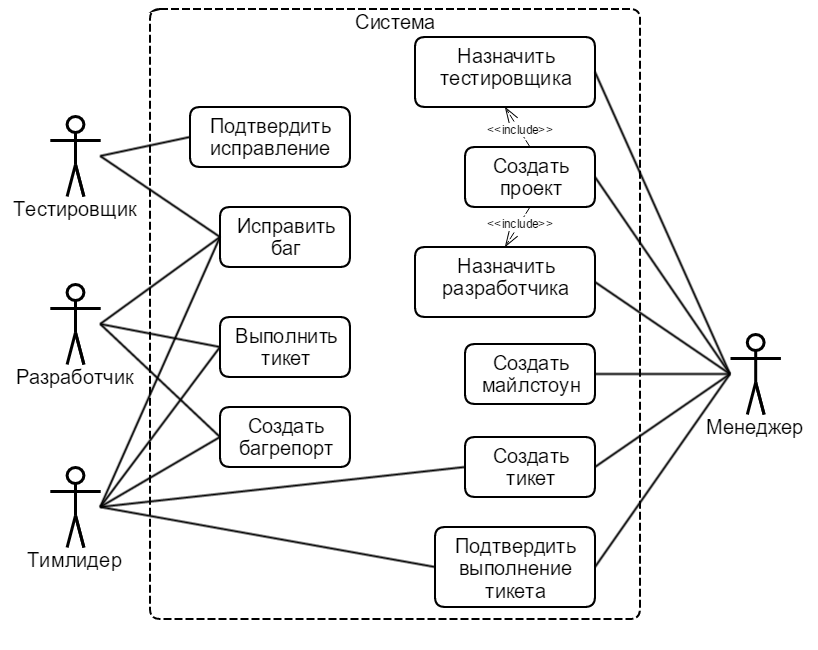
\includegraphics[width=\linewidth]{useCases}}
\caption{Варианты использования}
\label{fig:useCases}
\end{figure}

Разработка проекта:
\begin{itemize}
\item менеджер создает новый проект;
\item менеджер добавляет разработчиков в проект;
\item менеджер добавляет тестировщиков в проект;
\item менеджер определяет тимлидера;
\item менеджер определяет майлстоуны проекта и назначает даты;
\item менеджер выдает тикеты разработчикам;
\item разработчики выполняют тикеты ближайшего майлстоуна;
\item предыдущие три шага итеративно повторяются до завершения проекта;
\item проект завершается.
\end{itemize}

Выполнение тикета:
\begin{itemize}
\item менеджер/тимлидер создает новый тикет;
\item менеджер/тимлидер определяет разработчиков-исполнителей. Тикет получает статус "новый";
\item разработчик получает уведомление о новом тикете и меняет его статус на "принят";
\item разработчик приступает к выполнению задания. Тикет получает статус "в процессе выполнения";
\item разработчик выполняет задание и меняет статус тикета на "выполнен";
\item менеджер/тимлидер проверяет и подтверждает выполнение задания. Тикет получает задание "закрыт".
\end{itemize}

Обработка ошибки:
\begin{itemize}
\item разработчик/тестировщик создает отчет с описанием ошибки. Отчет получает статус "новый";
\item разработчик принимает уведомление и меняет статус отчета на "активен";
\item разработчик исправляет баг и меняет статус на "исправлен";
\item тестировщик проверяет исправление и закрывает отчета указав ему статус "закрыт".
\end{itemize}

%%%%%%%%%%%%%%%%%%%%%%%%%%%%%%%%%%%%%%%%%%%%%%%%%%%%%%%%%%%%%%%%%%%%%%%%%%%%%%%%%%%%%%%%%%%%%%%%%%%%%%
%%%%%%%%%%%%%%%%%%%%%%%%%%%%%%%%%%%%%%%%%%%%%%%%%%%%%%%%%%%%%%%%%%%%%%%%%%%%%%%%%%%%%%%%%%%%%%%%%%%%%%
\section{Динамическая объектная модель}
Диаграмма последовательности бизнес процесса разработки проекта приведена на рисунке~\ref{fig:sequenceProject}.
\begin{figure}[h]
\center{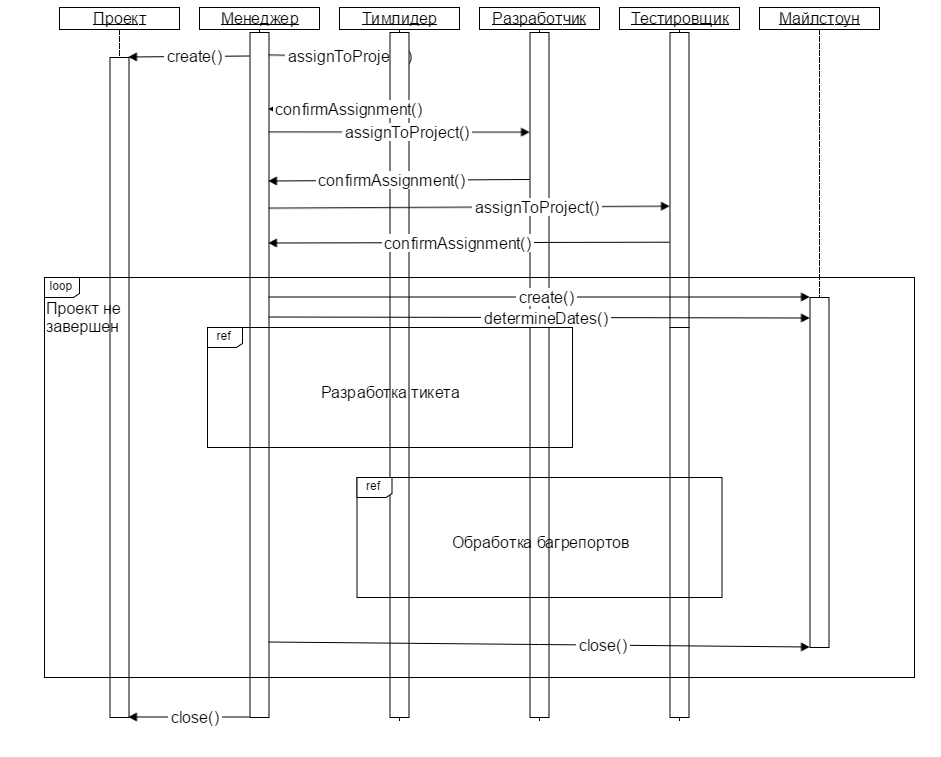
\includegraphics[width=\linewidth]{sequenceProject}}
\caption{Разработка проекта}
\label{fig:sequenceProject}
\end{figure}

Диаграмма последовательности бизнес процесса выполнения тикета приведена на рисунке~\ref{fig:sequenceTicket}.
\begin{figure}[h]
\center{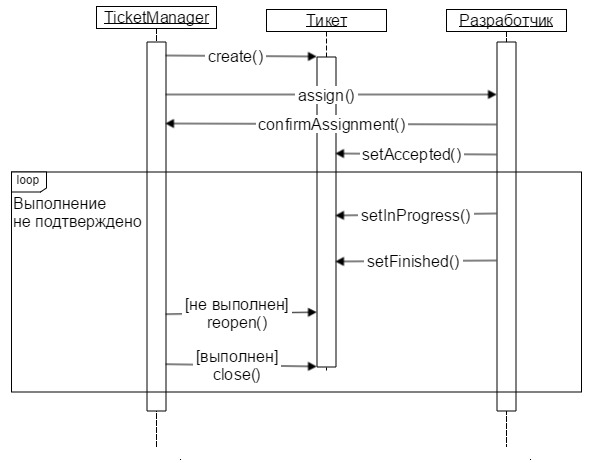
\includegraphics[width=\linewidth]{sequenceTicket}}
\caption{Выполнение тикета}
\label{fig:sequenceTicket}
\end{figure}

Диаграмма последовательности бизнес процесса исправления ошибки приведена на рисунке~\ref{fig:sequenceReport}.
\begin{figure}[h]
\center{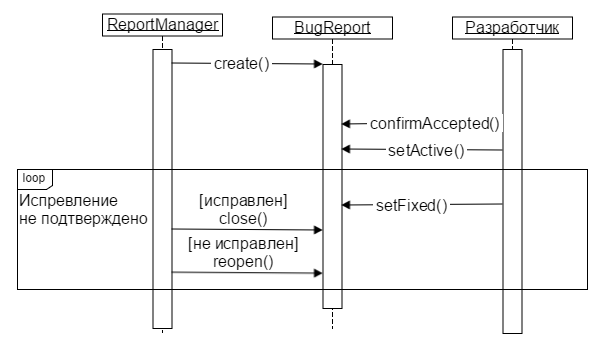
\includegraphics[width=\linewidth]{sequenceReport}}
\caption{Исправление ошибки}
\label{fig:sequenceReport}
\end{figure}

%%%%%%%%%%%%%%%%%%%%%%%%%%%%%%%%%%%%%%%%%%%%%%%%%%%%%%%%%%%%%%%%%%%%%%%%%%%%%%%%%%%%%%%%%%%%%%%%%%%%%%
%%%%%%%%%%%%%%%%%%%%%%%%%%%%%%%%%%%%%%%%%%%%%%%%%%%%%%%%%%%%%%%%%%%%%%%%%%%%%%%%%%%%%%%%%%%%%%%%%%%%%%
\section{Слой бизнес-логики}
Слой бизнес логики был реализован с помощью использования шаблона "Модель предметной области". Все классы, реализующий слой бизнес-логики разделены на два пакета:
\begin{itemize}
\item \texttt{entity} --- в данном пакете описаны все сущности, определенные в системе;
\item \texttt{logic} --- в данном пакете описаны все классы, реализующие бизнес-логику системы.
\end{itemize}

\subsection{Пакет \texttt{entity}}
В данном пакете описаны все сущности, над которыми оперирует бизнес-логика. Диаграмма классов пакета \texttt{entity} приведена на рисунке~\ref{fig:entityDiagram}.
\begin{figure}[h]
\center{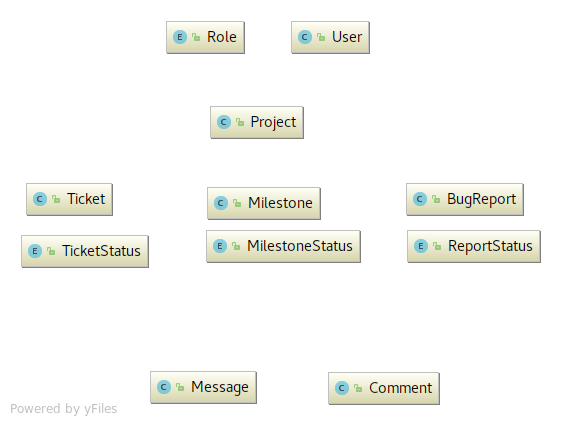
\includegraphics[width=\linewidth]{entityDiagram}}
\caption{Диаграмма классов пакета \texttt{entity}}
\label{fig:entityDiagram}
\end{figure}

Все классы данного пакета являются сущностными, т.е. они лишь хранят необходимые данные и имеют методы для получения/записи этих данных. Рассмотрим классы данного пакета более подробно.
\begin{itemize}
\item \texttt{User} --- класс, описывающий пользователя. Данный класс хранит: уникальный идентификатор пользователя; уникальный логин пользователя; имя; пароль и список уведомлений, полученных данным пользователем.

\item \texttt{Project} --- класс, описывающий проект. Данный класс хранит: уникальный идентификатор пользователя; уникальное имя проекта; указатель на менеджера проекта; указатель на тимлидера проекта~(если он определен); список разработчиков; список тестировщиков; список майлстоунов; список сообщений об ошибках.

\item \texttt{BugReport} --- класс, описывающий сообщение об ошибке. Данный класс хранит: уникальный идентификатор отчета; указатель на проект~(к которому он привязан); указатель на автора отчета об ошибке; указатель на разработчика, который исправляет данную ошибку~(если он определен); описание ошибки; список комментариев к данной ошибке.

\item \texttt{Milestone} --- класс, описывающий майлстоун. Класс хранит: уникальный идентификатор; проект, к которому привязан; текущий статус; предполагаемое время начало майлстоуна; время, когда майлстоун действительно был начат; предполагаемое время завершения майлстоуна; время, когда майлстоун был дейтсвительно завершен; список тикетов, привязанных к данному майлстоуну.

\item \texttt{Ticket} --- класс, описывающий тикет. Класс хранит: уникальный идентификатор; указатель на майлстоун, к которому привязан; указатель на создателя тикета; текущий статус; список разработчиков, назначенных на выполнение тикета; дату создания тикета; описание задания; список комментариев к данному тикету.

\item \texttt{Comment} --- класс, описывающий комментарий к тикету или отчету об ошибке. Класс хранит: уникальный идентификатор; дату создания комментария; указатель на пользователя, который оставил комментарий; текст комментария.

\item \texttt{Message} --- класс, описывающий уведомления пользователя. Класс хранит: уникальный идентификатор; дату создания уведомления; указатель на пользователя, которому отправлено уведомление; текст уведомления.
\end{itemize}

\subsection{Пакет \texttt{logic}}
В данном пакете описана вся бизнес-логика системы. Диаграмма классов пакета \texttt{logic} приведена на рисунке~\ref{fig:logicDiagram}.
\begin{figure}[h]
\center{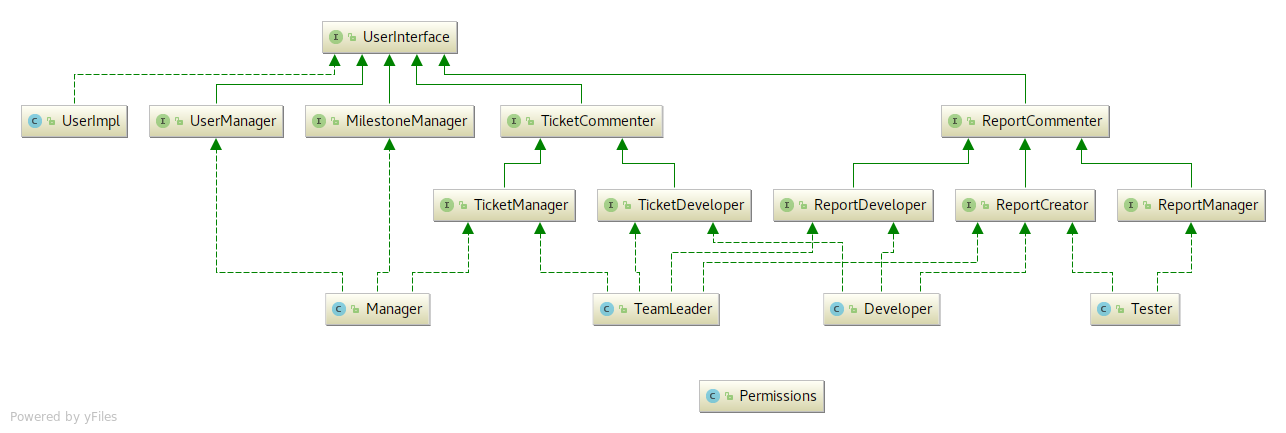
\includegraphics[width=\linewidth]{logicDiagram}}
\caption{Диаграмма классов пакета \texttt{logic}}
\label{fig:logicDiagram}
\end{figure}

Бизнес логика в данном пакете описывается на уровне интерфейсов, а классы соответствуют ролям и реализуют соответствующие интерфейсы. Рассмотрим их более подробно.

\begin{itemize}
\item \texttt{UserInterface} --- базовый интерфейс пользователя. Имеет методы:
	\begin{itemize}
	\item \texttt{getUser()} --- получить пользователя, к которому привязан текущий объект.
	\item \texttt{addMessage(String message)} --- добавить новое уведомление данному пользователю.
	\end{itemize}

\item \texttt{UserImpl} --- класс, который реализует базовый интерфейс пользователя.

\item \texttt{UserManager} --- интерфейс, в котором реализованы методы управления пользователями проекта. Расширяет интерфейс \texttt{UserInterface}. Методы могут выбросить два исключения: \texttt{MultipleRoleException} если какому-то пользователю пытаются присвоить две роли в проекте и \texttt{NoRightsException} если у текущего пользователя нет прав на управление пользователями проекта. Имеет методы:
	\begin{itemize}
	\item \texttt{setTeamLeader(Project project, User teamLeader)} --- добавить нового тимлидера к проекту.
	\item \texttt{addDeveloper(Project project, User developer)} --- добавить нового разработчика в проект.
	\item \texttt{addTester(Project project, User tester)} --- добавить нового тестировщика в проект.	
	\end{itemize}
	
\item \texttt{MilestoneManager} --- интерфейс, в котором реализованы методы управления майлстоуном. Расширяет интерфейс \texttt{UserInterface}. Имеет методы:
	\begin{itemize}
	\item \texttt{createMilestone(Project project, Date start, Date end)} --- добавить новый майлстоун в проект.
	\item \texttt{activateMilestone(Milestone milestone)} --- сделать майлстоун активным.
	\item \texttt{closeMilestone(Milestone milestone)} --- закрыть майлстоун.	
	\end{itemize}
	
	Выбрасывает следующие исключения:
	\begin{itemize}
	\item \texttt{NoRightsException} --- если у текущего пользователя нет прав на управление проектами.
	\item \texttt{TwoActiveMilestonesException} --- если пытаемся сделать одновременно два майлстоуна активными.
	\item \texttt{WrongStatusException} --- если пытаемся установить майлстоуну неправильный статус.	
	\item \texttt{MilestoneTicketNotClosedException} --- если пытаемся закрыть майлстоун, у которого закрыты не все тикеты.	
	\end{itemize}

\item \texttt{TicketCommenter} --- интерфейс, который реализует метод комментирования тикетов. Расширяет интерфейс \texttt{UserInterface}.
	
\item \texttt{TicketManager} --- интерфейс, в котором реализованы методы управления тикетом. Расширяет интерфейс \texttt{TicketCommenter}. Имеет методы:
	\begin{itemize}
	\item \texttt{checkTicketManagerPermissions(Ticket ticket)} --- проверить права текущего пользователя на управление данным тикетом.
	\item \texttt{createTicket(Milestone milestone, String task)} --- создать новый тикет.
	\item \texttt{addAssignee(Ticket ticket, User developer)} --- добавить нового разработчика в тикет.	
	\item \texttt{reopenTicket(Ticket ticket)} --- переоткрыть тикет.
	\item \texttt{closeTicket(Ticket ticket)} --- закрыть тикет.
	\end{itemize}
	
	Выбрасывает следующие исключения:
	\begin{itemize}
	\item \texttt{NoRightsException} --- если у текущего пользователя нет прав на управление тикетом.
	\item \texttt{MilestoneAlreadyClosedException} --- если пытаемся создать новый тикет в майлстоуне, который уже закрыт.
	\end{itemize}
	
\item \texttt{TicketDeveloper} --- интерфейс, в котором реализованы методы управления тикетом. Расширяет интерфейс \texttt{TicketCommenter}. Имеет методы:
	\begin{itemize}
	\item \texttt{checkTicketDeveloperPermissions(Ticket ticket)} --- проверить права текущего пользователя на разработку данного тикета.
	\item \texttt{acceptTicket(Ticket ticket)} --- поставить тикету статус "принят".
	\item \texttt{setInProgress(Ticket ticket)} --- поставить тикету статус "выполняется".	
	\item \texttt{finishTicket(Ticket ticket)} --- поставить тикету статус "завершен".
	\end{itemize}
	
	Выбрасывает исключение \texttt{NoRightsException} если у текущего пользователя нет прав на разработку тикета.

\item \texttt{ReportCommenter} --- интерфейс, который реализует метод комментирования отчетов об ошибках. Расширяет интерфейс \texttt{UserInterface}.

\item \texttt{ReportCreator} --- интерфейс, в котором реализованы методы создания отчетов об ошибках. Расширяет интерфейс \texttt{ReportCommenter}. Имеет методы:
	\begin{itemize}
	\item \texttt{checkReportCreatorPermissions(BugReport report)} --- проверить права текущего пользователя на создание отчетов об ошибках.
	\item \texttt{createReport(Project project, String description)} --- создать новый отчет об ошибке.
	\end{itemize}
	
	Выбрасывает исключение \texttt{NoRightsException} если у текущего пользователя нет прав на создание отчетов об ошибках.
	
\item \texttt{ReportDeveloper} --- интерфейс, в котором реализованы методы исправления ошибок проекта. Расширяет интерфейс \texttt{ReportCommenter}. Имеет методы:
	\begin{itemize}
	\item \texttt{checkReportDeveloperPermissions(BugReport report)} --- проверить права текущего пользователя на исправление ошибок проекта.
	\item \texttt{acceptReport(BugReport report)} --- принять отчет об ошибке на исправление.
	\item \texttt{fixReport(BugReport report)} --- установить статус "исправлен" отчету об ошибке.
	\end{itemize}
	
	Выбрасывает следующие исключения:
	\begin{itemize}
	\item \texttt{NoRightsException} --- если у текущего пользователя нет прав на исправление ошибок проекта.
	\item \texttt{AlreadyAcceptedException} --- если пытаемся принять на исправление отчет, который уже принят другим пользователем.
	\end{itemize}
	
\item \texttt{ReportManager} --- интерфейс, в котором реализованы методы управления отчетами об ошибках. Расширяет интерфейс \texttt{ReportCommenter}. Имеет методы:
	\begin{itemize}
	\item \texttt{checkReportManagerPermissions(BugReport report)} --- проверить права текущего пользователя на  управление отчетами об ошибках.
	\item \texttt{reopenReport(BugReport report)} --- переоткрыть отчет об ошибке, если она не была исправлена.
	\item \texttt{closeReport(BugReport report)} --- закрыть отчет об ошибке.
	\end{itemize}
	
	Выбрасывает исключение \texttt{NoRightsException} если у текущего пользователя нет прав на управление отчетами об ошибках.

\item \texttt{Manager} --- класс, который описывает роль менеджера проекта. Реализует интерфейсы \texttt{MilestoneManager}, \texttt{UserManager} и \texttt{TicketManager}.

\item \texttt{TeamLeader} --- класс, который описывает роль тимлидера проекта. Реализует интерфейсы \texttt{ReportCreator}, \texttt{ReportDeveloper}, \texttt{TicketManager}, \texttt{TicketDeveloper}.

\item \texttt{TeamLeader} --- класс, который описывает роль разработчика проекта. Реализует интерфейсы \texttt{ReportCreator}, \texttt{ReportDeveloper}, \texttt{TicketDeveloper}.

\item \texttt{TeamLeader} --- класс, который описывает роль тестировщика проекта. Реализует интерфейсы \texttt{ReportCreator}, \texttt{ReportManager}.

\item \texttt{Permissions} --- класс, который хранит права пользователя для какого-то проекта в виде битовой маски.
\end{itemize}

%%%%%%%%%%%%%%%%%%%%%%%%%%%%%%%%%%%%%%%%%%%%%%%%%%%%%%%%%%%%%%%%%%%%%%%%%%%%%%%%%%%%%%%%%%%%%%%%%%%%%%
%%%%%%%%%%%%%%%%%%%%%%%%%%%%%%%%%%%%%%%%%%%%%%%%%%%%%%%%%%%%%%%%%%%%%%%%%%%%%%%%%%%%%%%%%%%%%%%%%%%%%%
\section{Слой источников данных}
В качестве СУБД была выбрана система MySQL. Для работы с базой данных был использован Java Persistance API, в частности его реализация в библиотеке Hibernate. В базе данных хранятся все сущности, описанные в пакете \texttt{entity}. Описание сущностей производится с помощью специальных аннотаций JPA. Пример сущностного класса \texttt{User} приведен в листинге~\ref{lst:userORM}.
\begin{lstlisting}[style=crs_java, label={lst:userORM}, caption={Описание сущности}]
@Entity
@Table(name = "USERS")
public class User {

    @Id
    @Column(name = "ID")
    @GeneratedValue
    private Long id;

    @Column(name = "LOGIN", unique = true, nullable = false)
    private String login;

    @Column(name = "NAME")
    private String name;

    @Column(name = "PASSWORD")
    private String password;

    @JsonIgnore
    @OneToMany(fetch = FetchType.EAGER, mappedBy = "owner")
    private List<Message> messages = new ArrayList<>();
}
\end{lstlisting}

Также, для того чтобы Hibernate нашел все сущности, необходимо описать все сущностные классы в файле persistance.xml(листинг~\ref{lst:persistance}).
\begin{lstlisting}[style=crs_xml, label={lst:persistance}, caption={Файл persistance.xml}]
<?xml version="1.0" encoding="UTF-8" ?>
<persistence xmlns="http://java.sun.com/xml/ns/persistence"
             xmlns:xsi="http://www.w3.org/2001/XMLSchema-instance"
             xsi:schemaLocation="http://java.sun.com/xml/ns/persistence
 http://java.sun.com/xml/ns/persistence/persistence_1_0.xsd" version="1.0">

    <persistence-unit name="my-pms">
        <class>com.kspt.pms.entity.BugReport</class>
        <class>com.kspt.pms.entity.Comment</class>
        <class>com.kspt.pms.entity.Message</class>
        <class>com.kspt.pms.entity.Milestone</class>
        <class>com.kspt.pms.entity.Project</class>
        <class>com.kspt.pms.entity.Ticket</class>
        <class>com.kspt.pms.entity.User</class>
    </persistence-unit>

</persistence>
\end{lstlisting}

Для каждой сущности был реализован свой репозиторий, в котором определены методы для поиска и сохранения сущностей. Репозитории были реализованы с помощью библиотеки Spring Data. Данная библиотека позволяет описывать только интерфейс, и по названиям методов этого интерфейса умеет автоматически генерировать его реализацию. Это очень сильно упрощает работу с базой данных. Рассмотрим данные репозитории более подробно.
\begin{itemize}
\item \texttt{BugReportRepository}
	\begin{itemize}
	\item \texttt{Optional<BugReport> findById(Long id)} --- поиск по идентификатору.
	\item \texttt{Collection<BugReport> findByProjectName(String name)} --- поиск всех отчетов, принадлежащих проекту с заданным именем.
	\item \texttt{Collection<BugReport> findByCreatorLogin(String login)} --- поиск всех отчетов, созданных пользователем с заданным логином.
	\item \texttt{Collection<BugReport> findByDeveloperLogin(String login)} --- поиск всех отчетов, исправляемых пользователем с заданным логином.	
	\end{itemize}
	
\item \texttt{CommentRepository}
	\begin{itemize}
	\item \texttt{Optional<Comment> findById(Long id)} --- поиск по идентификатору.
	\item \texttt{Collection<Comment> findByUserLogin(String login)} --- поиск всех комментариев, оставленных пользователем с заданным логином.
	\end{itemize}
	
\item \texttt{MessageRepository}
	\begin{itemize}
	\item \texttt{Collection<Message> findByOwnerLogin(String login)} --- поиск всех уведомлений, принадлежащих пользователю с заданным логином.
	\end{itemize}
	
\item \texttt{MilestoneRepository}
	\begin{itemize}
	\item \texttt{Optional<Milestone> findById(Long id)} --- поиск по идентификатору.
	\item \texttt{Collection<Milestone> findByProjectName(String name)} --- поиск всех майлстоуну, принадлежащих проекту с заданным именем.
	\end{itemize}
	
\item \texttt{ProjectRepository}
	\begin{itemize}
	\item \texttt{Optional<Project> findByName(String name)} --- поиск по имени.
	\item \texttt{Collection<Project> findByManagerLogin(String login)} --- поиск по менеджеру.
	\item \texttt{Collection<Project> findByTeamLeaderLogin(String login)} --- поиск по тимлидеру.
	\item \texttt{Collection<Project> findByDevelopersContaining(User user)} --- поиск по разработчику.
	\item \texttt{Collection<Project> findByTestersContaining(User user)} --- поиск по тестировщику.
	\end{itemize}
	
\item \texttt{TicketRepository}
	\begin{itemize}
	\item \texttt{Optional<Ticket> findById(Long id)} --- поиск по идентификатору.
	\item \texttt{Collection<Ticket> findByMilestoneId(Long id)} --- поиск майлстоуну.
	\item \texttt{Collection<Ticket> findByAssigneesContaining(User user)} --- поиск по исполнителю.
	\item \texttt{Collection<Ticket> findByCreatorLogin(String login)} --- поиск по создателю.
	\end{itemize}
	
\item \texttt{UserRepository}
	\begin{itemize}
	\item \texttt{Optional<User> findByLogin(String login)} --- поиск по логину.
	\end{itemize}
\end{itemize}

Для того, чтобы все эти библиотеки правильно проинициализировались, необходимо в классе конфигурации определить источник данных~(листинг~\ref{lst:config}).
\begin{lstlisting}[style=crs_java, label={lst:config}, caption={Конфигурация источника данных}]
    @Bean
    public DataSource dataSource() {
        DriverManagerDataSource dataSource = new DriverManagerDataSource();
        dataSource.setDriverClassName(env.getRequiredProperty("jdbc.driverClassName"));
        dataSource.setUrl(env.getRequiredProperty("jdbc.url"));
        dataSource.setUsername(env.getRequiredProperty("jdbc.username"));
        dataSource.setPassword(env.getRequiredProperty("jdbc.password"));
        return dataSource;
    }

    @Bean
    public JdbcTemplate jdbcTemplate(DataSource dataSource) {
        JdbcTemplate jdbcTemplate = new JdbcTemplate(dataSource);
        jdbcTemplate.setResultsMapCaseInsensitive(true);
        return jdbcTemplate;
    }

    public Properties additionalProreties() {
        Properties properties = new Properties();
//        properties.setProperty("hibernate.show_sql", "true");
        return properties;
    }
    
    @Bean
    public EntityManagerFactory entityManagerFactory() {
        HibernateJpaVendorAdapter vendorAdapter = new HibernateJpaVendorAdapter();
        vendorAdapter.setGenerateDdl(true);

        LocalContainerEntityManagerFactoryBean factory = new LocalContainerEntityManagerFactoryBean();
        factory.setJpaVendorAdapter(vendorAdapter);
        factory.setPackagesToScan("com.kspt.pms");
        factory.setDataSource(dataSource());
        factory.setPersistenceUnitName("my-pms");
        factory.setPersistenceProviderClass(HibernatePersistenceProvider.class);
        factory.setJpaProperties(additionalProreties());
        factory.afterPropertiesSet();
        return factory.getObject();
    }

    @Bean
    public PlatformTransactionManager transactionManager() {
        JpaTransactionManager txManager = new JpaTransactionManager();
        txManager.setEntityManagerFactory(entityManagerFactory());
        return txManager;
    }
\end{lstlisting}

%%%%%%%%%%%%%%%%%%%%%%%%%%%%%%%%%%%%%%%%%%%%%%%%%%%%%%%%%%%%%%%%%%%%%%%%%%%%%%%%%%%%%%%%%%%%%%%%%%%%%%
%%%%%%%%%%%%%%%%%%%%%%%%%%%%%%%%%%%%%%%%%%%%%%%%%%%%%%%%%%%%%%%%%%%%%%%%%%%%%%%%%%%%%%%%%%%%%%%%%%%%%%
\section{Слой представления}

В качестве фреймворка для слоя представления была выбрана технология Spring MVC. Данная технология позволяет реализовать паттерн Model-View-Controller при помощи слабо связанных компонентов. В качестве модели выступает слой бизнес-логики приложения. Контроллеры реализованы в виде RESTful контроллеров с помощью фреймворка Spring. Представление реализовано с помощью JavaScript фреймворка AngularJS и HTML страниц. Работа происходит по следующему сценарию:
\begin{enumerate}
\item RESTful сервис принимает запрос от пользователя;
\item сервис вызывает соответствующие методы бизнес логики для обработки запроса;
\item сервис возвращает ответ на запрос в виде JSON-объекта;
\item AngularJS клиент получает ответ от сервера и рэндерит соответствующую HTML-страницу и показывает его в браузере.
\end{enumerate}

Рассмотрим более подробно REST API, предоставляемый сервером.
\begin{itemize}
\item \texttt{UserController}
	\begin{itemize}
	\item URL: \texttt{"rest/user/:login"} --- получение пользователя с логином \texttt{login}
	\item URL: \texttt{"rest/user/:login"}, метод POST --- регистрация нового пользователя
	\item URL: \texttt{"rest/user/:login/authenticate"} --- аутентификация пользователя
	\item URL: \texttt{"rest/user/:login/messages"} --- получить все уведомления для пользователя
	\item URL: \texttt{"rest/user/:login/projects"} --- получить все проекты, в которых участвует пользователя
	\item URL: \texttt{"rest/user/:login/projects"}, метод POST --- добавление нового проекта пользователю
	\item URL: \texttt{"rest/user/:login/managed\_tickets"} --- получить все тикеты, которыми руководит пользователь
	\item URL: \texttt{"rest/user/:login/assigned\_tickets"} --- получить все тикеты, которые разрабатывает пользователь
	\item URL: \texttt{"rest/user/:login/managed\_reports"} --- получить все ошибки, которыми руководит пользователь
	\item URL: \texttt{"rest/user/:login/assigned\_reports"} --- получить все ошибки, которые разрабатывает пользователь
	\end{itemize}
	
\item \texttt{TicketController}
	\begin{itemize}
	\item URL: \texttt{"rest/ticket/:id"} --- получение тикета с идентификатором \texttt{id}
	\item URL: \texttt{"rest/ticket/:id/permissions"} --- получение прав пользователя для тикета
	\item URL: \texttt{"rest/ticket/:id/milestone"} --- получение майлстоуна тикета
	\item URL: \texttt{"rest/ticket/:id"}, метод PUT --- установить новый статус тикету
	\item URL: \texttt{"rest/ticket/:id/assignees"} --- получить всех разработчиков тикета
	\item URL: \texttt{"rest/ticket/:id/assignees"}, метод POST --- добавить нового разработчика в тикет
	\item URL: \texttt{"rest/ticket/:id/comments"} --- получить все комментарии тикета
	\item URL: \texttt{"rest/ticket/:id/comments"}, метод POST --- добавить новый комментарий тикету
	\end{itemize}
	
\item \texttt{ReportController}
	\begin{itemize}
	\item URL: \texttt{"rest/report/:id"} --- получение отчета с идентификатором \texttt{id}
	\item URL: \texttt{"rest/report/:id/permissions"} --- получение прав пользователя для отчета
	\item URL: \texttt{"rest/report/:id/project"} --- получение проекта отчета
	\item URL: \texttt{"rest/report/:id"}, метод PUT --- установить новый статус отчету
	\item URL: \texttt{"rest/report/:id/comments"} --- получить все комментарии отчета
	\item URL: \texttt{"rest/report/:id/comments"}, метод POST --- добавить новый комментарий отчету
	\end{itemize}
	
\item \texttt{ProjectController}
	\begin{itemize}
	\item URL: \texttt{"rest/project/:name"} --- получение проекта с именем \texttt{name}
	\item URL: \texttt{"rest/project/:name"}, метод PUT --- обновить проект с именем \texttt{name}
	\item URL: \texttt{"rest/project/:name/permissions"} --- получение прав для проекта
	\item URL: \texttt{"rest/project/:name/reports"} --- получение ошибок для проекта
	\item URL: \texttt{"rest/project/:name/reports"}, метод POST --- добавление ошибки в проект
	\item URL: \texttt{"rest/project/:name/milestones"} --- получение майлстоунов для проекта
	\item URL: \texttt{"rest/project/:name/milestones"}, метод POST --- добавление майлстоуна в проект
	\item URL: \texttt{"rest/project/:name/developers"} --- получение разработчиков проекта
	\item URL: \texttt{"rest/project/:name/developers"}, метод POST --- добавление разработчика в проект
	\item URL: \texttt{"rest/project/:name/testers"} --- получение тестировщиков проекта
	\item URL: \texttt{"rest/project/:name/testers"}, метод POST --- добавление тестировщика в проект
	\end{itemize}
	
\item \texttt{MilestoneController}
	\begin{itemize}
	\item URL: \texttt{"rest/milestone/:id"} --- получение майлстоуна с идентификатором \texttt{id}
	\item URL: \texttt{"rest/milestone/:id/permissions"} --- получение прав пользователя для майлстоуна
	\item URL: \texttt{"rest/milestone/:id/project"} --- получение проекта майлстоуна
	\item URL: \texttt{"rest/milestone/:id"}, метод PUT --- установить новый статус майлстоуну
	\item URL: \texttt{"rest/milestone/:id/tickets"} --- получить все тикеты майлстоуна
	\item URL: \texttt{"rest/milestone/:id/tickets"}, метод POST --- добавить новый тикеты майлстоуну
	\end{itemize}	
\end{itemize}

При возникновении неполадок на стороне сервера, выбрасывается соответствующее исключение. Данное исключение перехватывается с помощью специальных инструментов и генерируется HTTP ответ, который содержит код и сообщение с описанием ошибки.

Клиентская сторона посылает запросы к соответствующим RESTful сервисам и затем рэндерит соответствующую HTML страницу. Работа с REST API происходит с помощью библиотеки Angular Resource. Пример angular-контроллера приведен на листинге
\begin{lstlisting}[style=crs_js, label={lst:jsController}, caption={Angular-контроллер}]
/**
 * Created by kivi on 18.12.17.
 */

function ReportService($resource) {
    return $resource('rest/report/:id', {id: '@id'});
}

function ReportPermService($resource) {
    return $resource('rest/report/:id/permissions?user=:login', {id: '@id', login: '@login'});
}

function ReportProjectService($resource) {
    return $resource('rest/report/:id/project', {id: '@id'});
}

function ReportCommentService($resource) {
    return $resource('rest/report/:id/comments?user=:login', {id: '@id', login: '@login'});
}

function ReportController($scope, $http, $routeParams,
                          ReportService,
                          ReportPermService,
                          ReportCommentService,
                          ReportProjectService,
                          InfoShareService) {
    function url() {
        return {id: $routeParams.id};
    }
    function url_with_login(login) {
        return {id: $routeParams.id, login:login};
    }

    this.user = InfoShareService.getUser();
    this.permissions = ReportPermService.get(url_with_login(this.user.login));
    this.project = ReportProjectService.get(url());
    this.instance = ReportService.get(url());
    this.comments = ReportCommentService.query(url());

    this.changeStatus = function (status) {
        $http.put('rest/report/' + this.instance.id + '?user=' + this.user.login, status)
            .then(function () {
                this.update();
            }.bind(this), function (error) {
                alert(error.data.message);
        });
    };

    this.commentReport = function () {
        if (isEmpty($scope.reportComment)) {
            alert("Enter comment message");
        } else {
            var comment = new ReportCommentService();
            comment.description = $scope.reportComment;
            comment.$save(url_with_login(this.user.login), function () {
                $scope.reportComment = "";
                this.updateComments();
            }.bind(this), function (error) {
                alert(error.data.message);
            });
        }
    };

    this.update = function () {
        this.instance = ReportService.get(url());
    };

    this.updateComments = function () {
        this.comments = ReportCommentService.query(url());
    }
}

app
    .factory('ReportService', ReportService)
    .factory('ReportPermService', ReportPermService)
    .factory('ReportProjectService', ReportProjectService)
    .factory('ReportCommentService', ReportCommentService)
    .controller('ReportController', ReportController);
\end{lstlisting}

Скриншоты пользовательского интерфейса приведены на рисунках~\ref{fig:loginPage} -- \ref{fig:reportPage}.

\begin{figure}[h]
\center{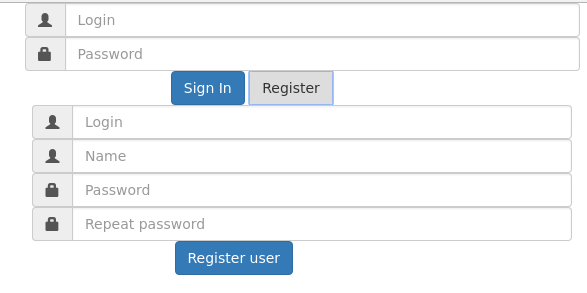
\includegraphics[width=\linewidth]{loginPage}}
\caption{Страница входа}
\label{fig:loginPage}
\end{figure}
\begin{figure}[h]
\center{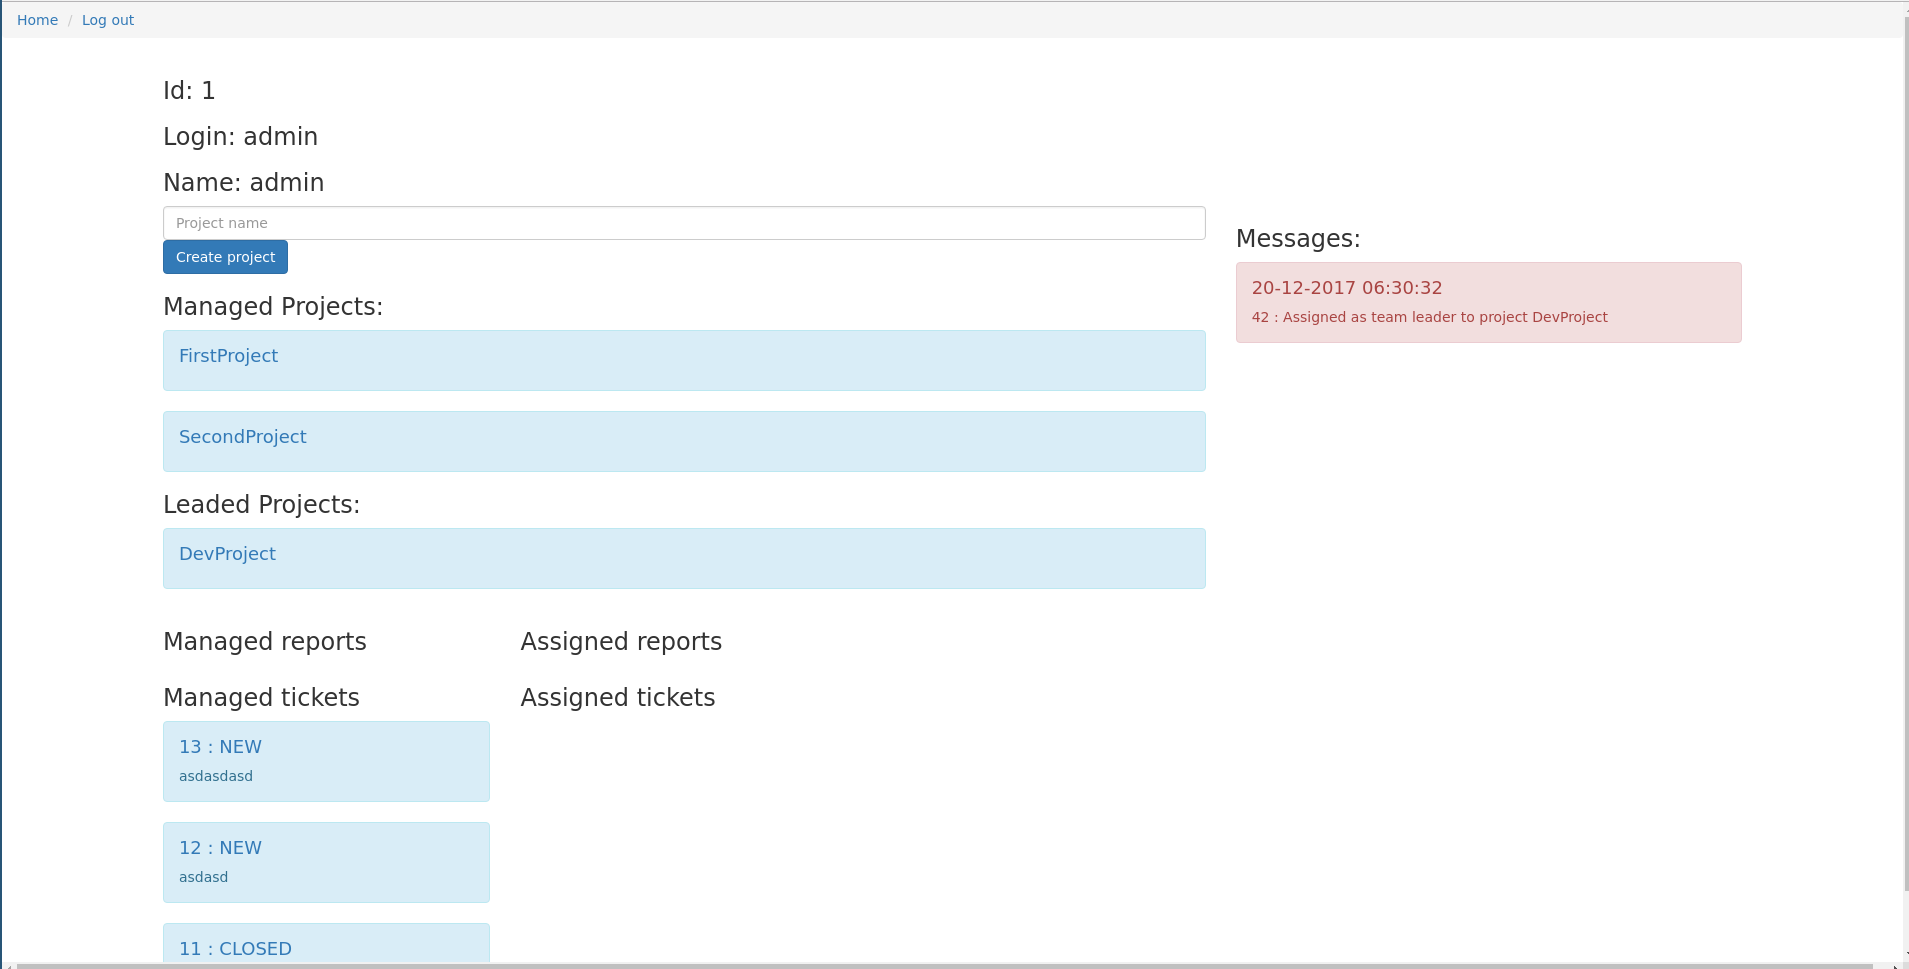
\includegraphics[width=\linewidth]{userPage}}
\caption{Страница пользователя}
\label{fig:userPage}
\end{figure}
\begin{figure}[h]
\center{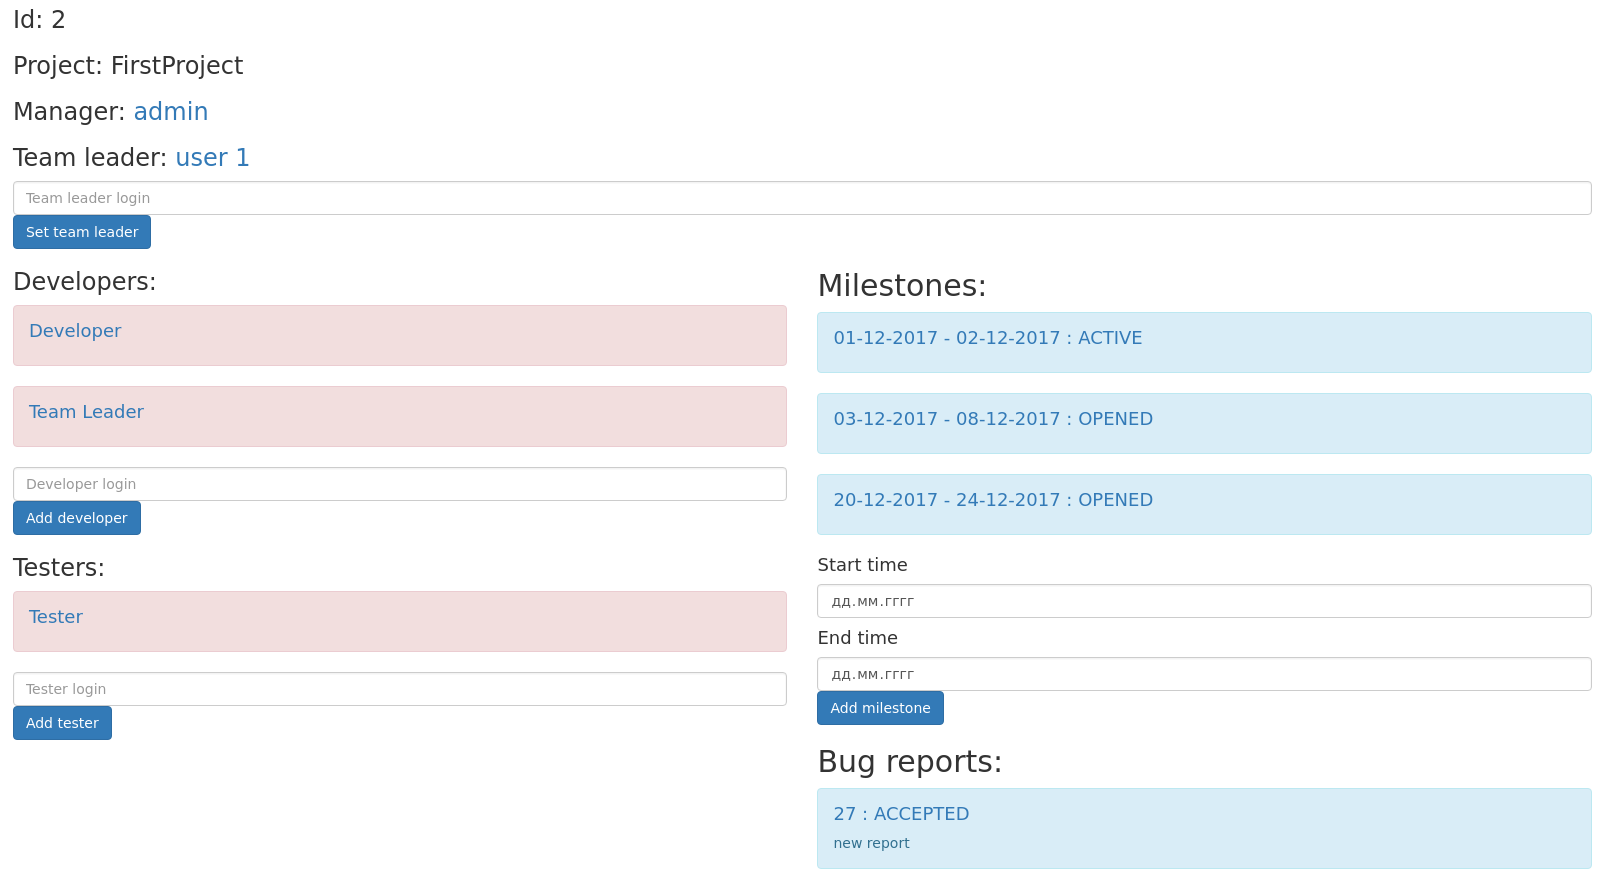
\includegraphics[width=\linewidth]{projectPage}}
\caption{Страница проекта}
\label{fig:projectPage}
\end{figure}
\begin{figure}[h]
\center{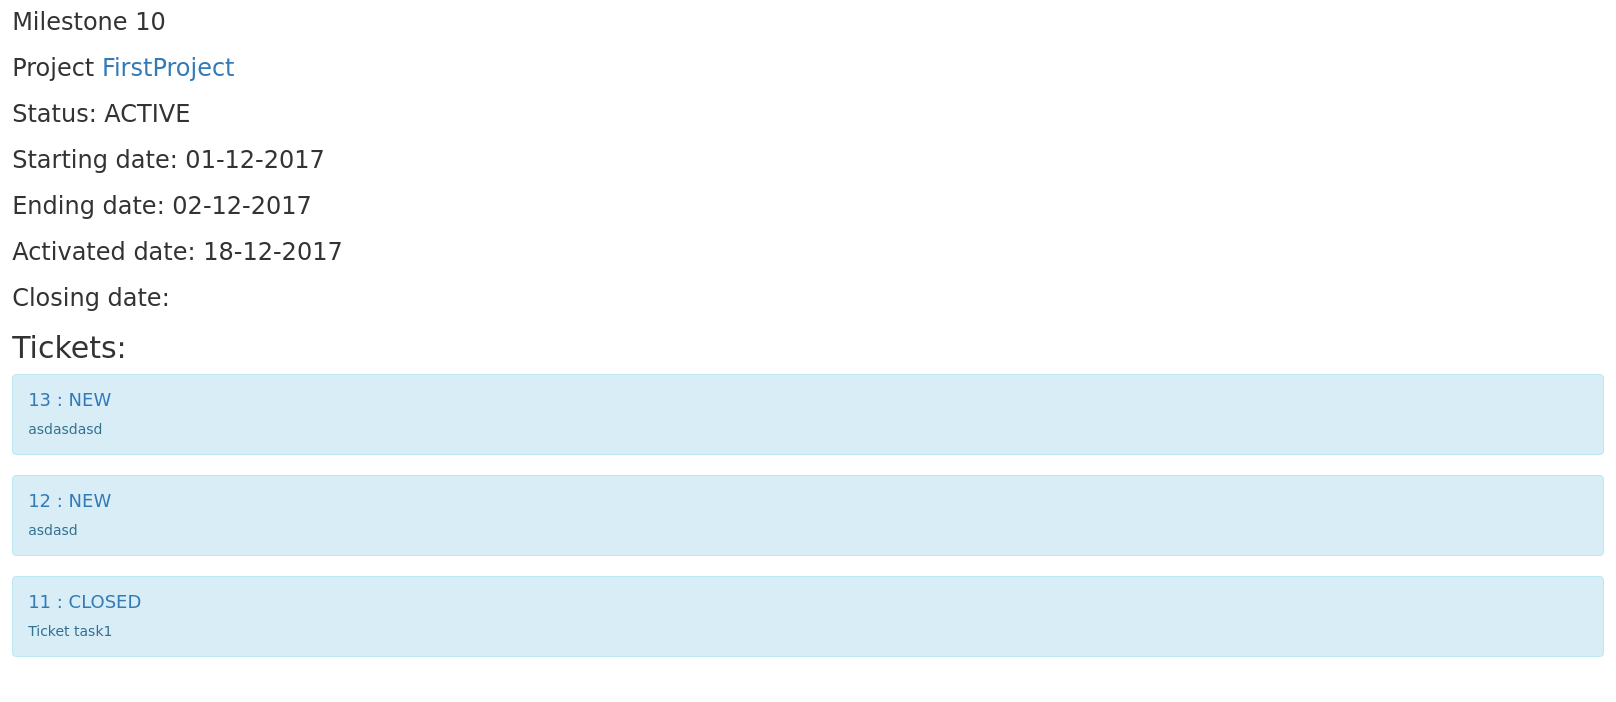
\includegraphics[width=\linewidth]{milestonePage}}
\caption{Страница майлстоуна}
\label{fig:milestonePage}
\end{figure}
\begin{figure}[h]
\center{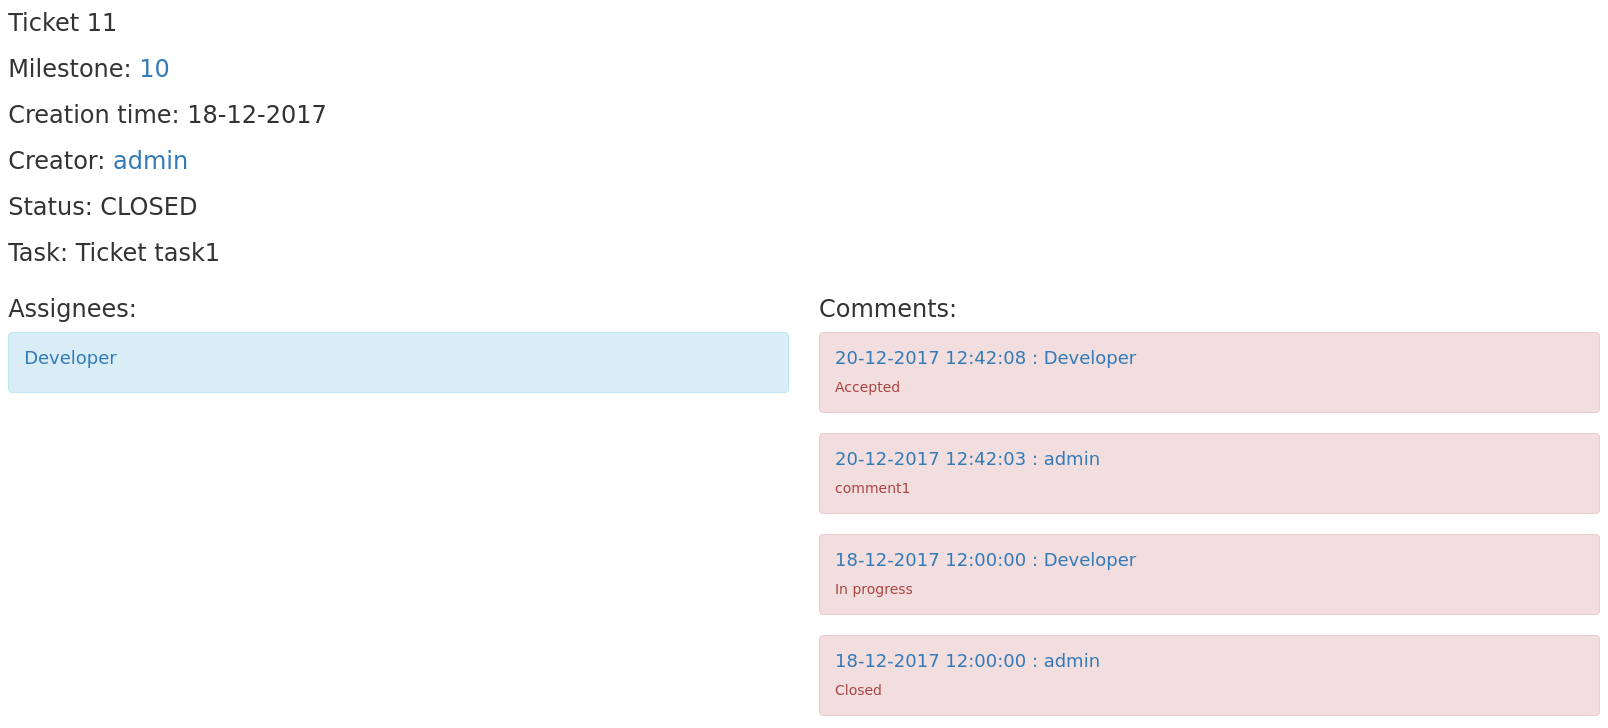
\includegraphics[width=\linewidth]{ticketPage}}
\caption{Страница тикета}
\label{fig:ticketPage}
\end{figure}
\begin{figure}[h]
\center{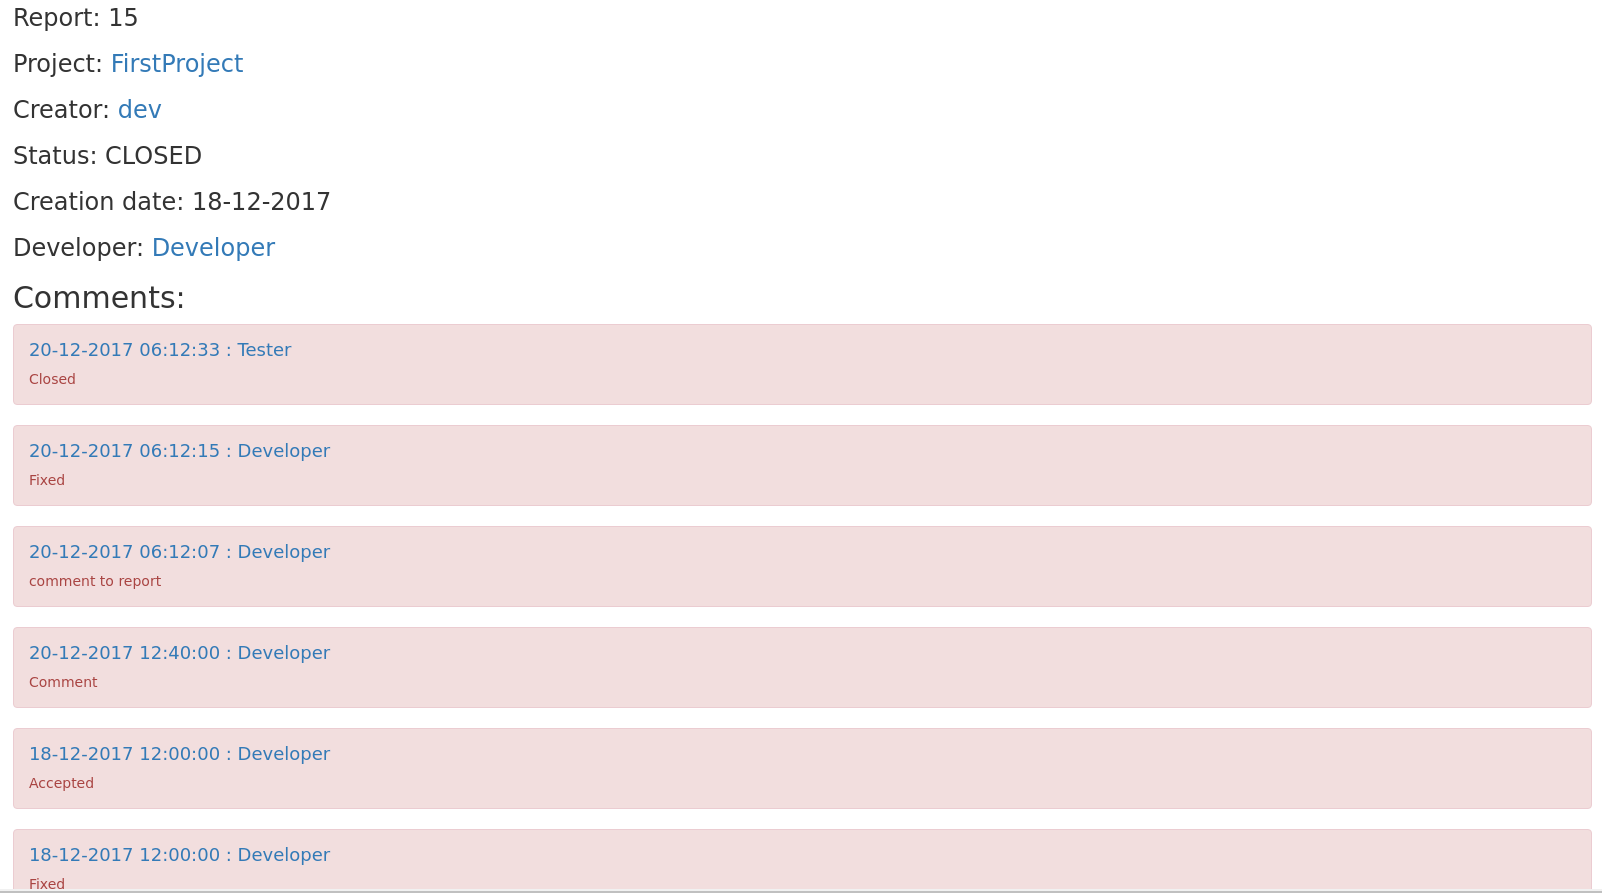
\includegraphics[width=\linewidth]{reportPage}}
\caption{Страница отчета об ошибке}
\label{fig:reportPage}
\end{figure}

%%%%%%%%%%%%%%%%%%%%%%%%%%%%%%%%%%%%%%%%%%%%%%%%%%%%%%%%%%%%%%%%%%%%%%%%%%%%%%%%%%%%%%%%%%%%%%%%%%%%%%
%%%%%%%%%%%%%%%%%%%%%%%%%%%%%%%%%%%%%%%%%%%%%%%%%%%%%%%%%%%%%%%%%%%%%%%%%%%%%%%%%%%%%%%%%%%%%%%%%%%%%%
\section{Тестирование}

Было проведено ручное функциональное тестирование приложения. Были протестированы все бизнес-процессы в приложении, проверена обработка ошибочных ситуаций. Список проводимых тестов:
\begin{itemize}
\item \textbf{Попытка добавить пользователя, который уже существует}. Окрываем окно регистрации нового пользователя, вводим данные пользователя. В поле \texttt{Login} указываем логин уже зарегистрированного пользователя. Нажимаем кнопку \texttt{Register}. В результате появится окно с сообщением <<User \texttt{login} already exists>>.

\item \textbf{Регистрация нового пользователя}. Открыть окно регистрации пользователя. Ввести уникальные данные пользователя. Нажать кнопку \texttt{Register}. Регистрация должна пройти успешно. Должно отрыться окно входа в систему.

\item \textbf{Попытка войти в систему с неправильным логином или паролем}. В окне входа в систему ввести неправильные данные пользователя (логин или пароль). Нажать кнопку \texttt{Sign In}. Должно появиться окно с сообщением <<Incorrect login or password>>.

\item \textbf{Вход в систему}. В окне входа в систему ввести правильные данные пользователя. Нажать кнопку \texttt{Sign In}. Должно открыться окно указанного пользователя.

\item \textbf{Создание проекта с дублирующимся именем}. В окне пользователя в строке добавления нового проекта ввести имя нового проекта, которое полностью совпадает с именем уже существующего проекта. Нажать кнопку \texttt{Create project}. Должно появиться окно ошибки с сообщением <<Project \texttt{name} already exists>>.

\item \textbf{Создание нового проекта}. В окне пользователя в строке добавления нового проекта ввести уникальное имя нового проекта. Нажать кнопку \texttt{Create project}. В списке <<Managed projects>> должен появиться новый проект с указанным именем.

\item \textbf{Установка несуществующего пользователя тимлидером}. Открыть окно нового проекта. Должна быть доступна кнопка \texttt{Set team leader}. Ввести несуществующий логин пользователя и нажать на кнопку. Должно появиться окно ошибки с сообщением <<User \texttt{login} not found>>.

\item \textbf{Назначение тимлидера}. Ввести данные существующего пользователя и нажать на кнопку \texttt{Set team leader}. Операция должна успешно завершиться. В окне проекта возле пункта \texttt{Team leader} должно появиться имя указанного пользователя.

\item \textbf{Добавление участников в проект}.
	\begin{itemize}
	\item В окне проекта под списком разрабочиков ввести логин несуществующего пользователя и нажать кнопку \texttt{Add developer}. Должно появиться окно ошибки с сообщением <<User \texttt{login} not found>>.
	\item В окне проекта под списком разрабочиков ввести логин тимлидера проекта и нажать кнопку \texttt{Add developer}. Должно появиться окно ошибки с сообщением <<User \texttt{login} already have a role \texttt{role} in project \texttt{name}>>.
	\item В окне проекта под списком разрабочиков ввести логин существующего пользователя и нажать кнопку \texttt{Add developer}. Операция должна завершиться успешно. В списке разработчиков должна появиться новая строчка с именем указанного пользователя.
	\item В окне проекта под списком тестировщиков ввести логин несуществующего пользователя и нажать кнопку \texttt{Add tester}. Должно появиться окно ошибки с сообщением <<User \texttt{login} not found>>.
	\item В окне проекта под списком тестировщиков ввести логин тимлидера проекта и нажать кнопку \texttt{Add tester}. Должно появиться окно ошибки с сообщением <<User \texttt{login} already have a role \texttt{role} in project \texttt{name}>>.
	\item В окне проекта под списком тестировщиков ввести логин существующего пользователя и нажать кнопку \texttt{Add tester}. Операция должна завершиться успешно. В списке тестировщиков должна появиться новая строчка с именем указанного пользователя.
	\end{itemize}

\item \textbf{Добавление майлстоуна, у которого дата завершения раньше чем дата начала}. В окне проекта под списком майлстоунов ввести даты начала и завершения майлстоуна так, чтобы дата завершения была перед датой начала. Нажать \texttt{Add milestone}. Должно появиться окно ошибки с сообщением <<Can't create milestone with end date before start date>>.

\item \textbf{Добавление майлстоуна, у которого дата завершения в прошлом}. В окне проекта под списком майлстоунов ввести даты начала и завершения майлстоуна так, чтобы дата завершения была в прошлом. Нажать \texttt{Add milestone}. Должно появиться окно ошибки с сообщением <<Can't create milestone with end date in the past>>.

\item \textbf{Добавление майлстоуна}. В окне проекта под списком майлстоунов ввести корректные даты начала и завершения майлстоуна. Нажать \texttt{Add milestone}. В списке майлстоунов проекта должна появиться новая запись, соответствующая созданному майлстоуну. Статус появившегося майлстоуна --- <<OPENED>>.

\item \textbf{Неправильная смена статуса майлстоуна}. Открыть окно нового майлстоуна. Попытаться изменить статус майлстоуна с <<OPENED>> на <<CLOSED>> нажав на кнопку \texttt{Close}. Должно появиться окно ошибки с сообщением <<Cannot change status from OPENED to CLOSED>>.

\item \textbf{Добвление тикета}. В окне майлстоуна ввести описание нового тикета и нажать на кнопку \texttt{Add ticket}. В списке тикетов майлстоуна должна появиться новая строчка с описанием созданного тикета.

\item \textbf{Активация майлстоуна}. В окне нового майлстоуна нажать кнопку \texttt{Activate}. Операция должна пройти успешно. Статус майлстоуна должен поменяться на <<ACTIVE>>. В окне майлстоуна справа от строчки \texttt{Activated date} должна появиться текущая дата.

\item \textbf{Два активных майлстоуна одновременно}. В окне проекта создать новый майлстоун. Открыть окно нового майлстоуна и нажать кнопку \texttt{Activate}. Должно появиться окно ошибки с сообщением <<Attempting to activate milestone \texttt{id1}, when milestone \texttt{id2} is already active>>.

\item \textbf{Закрыть майлстоун когда не все его тикеты закрыты}. Окрыть окно активного майлстоуна. Нажать кнопку \texttt{Close}. Должно появиться окно ошибки с сообщением <<Ticket \texttt{id} is not closed>>.

\item \textbf{Добавить разработчика в тикет}. Открыть окно нового тикета. Под списком разработчиков вести логин разработчика, являющегося разработчиком в проекте. Нажать \texttt{Add assignee}. В списке разработчиков тикета должна появиться новая строчка с именем указанного пользователя.

\item \textbf{Добавить неправильного пользователя в проект}. В окне тикета ввести логин пользователя, который существует в системе но никак не связан с проектом. Нажать \texttt{Add assignee}. Должно появиться окно ошибки с сообщением <<User \texttt{login} has no permission \texttt{permission} for project \texttt{name}>>.

\item \textbf{Проверка добавления разработчика}. Выйти из аккаунта менеджера. Войти в всистему за пользователя, которого только что назначили разработчиком тикета. В главном окне пользователя быть одна запись в списке разрабатываемых тикетов --- созданный ранее тикет.

\item \textbf{Поменять статус тикета на <<ACCEPTED>>}. Октрыть окно тикета. Нажать на кнопку \texttt{Set accepted}. Статус тикета должен поменяться. В списке комментариев тикета должна появиться соответствующая запись.

\item \textbf{Поменять статус тикета на <<IN\_PROGRESS>>}. Октрыть окно тикета. Нажать на кнопку \texttt{Set in progress}. Статус тикета должен поменяться. В таблице комментариев тикета должна появиться соответствующая запись.

\item \textbf{Поменять статус тикета на <<FINISHED>>}. Октрыть окно тикета. Нажать на кнопку \texttt{Set finished}. Статус тикета должен поменяться. В таблице комментариев тикета должна появиться соответствующая запись.

\item \textbf{Закрыть тикет}. Выйти из системы. Войти в систему за пользователя \texttt{manager}. Открыть окно тикета. Нажать на кнопку \texttt{Set closed}. Статус тикета должен поменяться. В таблице комментариев тикета должна появиться соответствующая запись.

\item \textbf{Закрыть майлстоун}. Открыть окно майлстоуна, к которому был привязан тикет. Нажать на кнопку \texttt{Close}. Операция должна завершиться успешно. Статус майлстоуна должен поменяться на <<CLOSED>>. В окне майлстоуна справа от строчки \texttt{Closing date} должна появиться текущая дата.

\item \textbf{Добавить тикет в закрытый майлстоун}. Открыть окно закрытого майлстоуна. Ввести описание нового тикета и нажать на кнопку \texttt{Add ticket}. Должно появиться окно ошибки с сообщением <<Milestone \texttt{id} of project \texttt{name} is already closed>>.

\item \textbf{Создать багрепорт}. Выйти из системы. Войти в систему за пользователя \texttt{teamleader}. Открыть окно проекта. Ввести описание ошибки и нажать на кнопку \texttt{Add report}. В списке ошибок должна появиться новая строчка, соответствующая созданному ошибок.

\item \textbf{Принять багрепорт}. Выйти из системы. Войти в систему за пользователя \texttt{developer}. Открыть окно багрепорта. Поменять статус на <<ACCEPTED>>. Статус багрепорта должен поменяться. В таблице комментариев должен появиться соответствующий комментарий. На странице багрепорта справа от пункта \texttt{Developer} должно появиться имя текущего пользователя.

\item \textbf{Принять принятый багрепорт}. Выйти из системы. Войти в систему за пользователя \texttt{teamleader}. Открыть окно багрепорта. Пoменять статус на <<ACCEPTED>>. Должно появиться окно ошибки с сообщением, что другой пользователь уже принял этот багрепорт.

\item \textbf{Багрепорты разработчика}. Выйти из системы. Войти в систему за пользователя \texttt{developer}. В списке разрабатываемых багрепортов на странице пользователя должна появиться запись, соответствующая принятому багрепорту.

\item \textbf{Исправить багрепорт}. Открыть окно багрепорта. Поменять статус на <<FIXED>>. Статус багрепорта должен поменяться. В таблице комментариев должен появиться соответствующий комментарий.

\item \textbf{Переоткрыть багрепорт}. Выйти из системы. Войти в систему за пользователя \texttt{tester}. Открыть окно багрепорта. Поменять статус на <<OPENED>>. Статус багрепорта должен поменяться. В таблице комментариев должен появиться соответствующий комментарий.

\item \textbf{Снова исправить багрепорт}. Выйти из системы. Войти в систему за пользователя \texttt{developer}. Открыть окно багрепорта. Поменять статус на <<FIXED>>. В появившемся окне ввести комментарий. Статус багрепорта должен поменяться. В таблице комментариев должен появиться соответствующий комментарий.

\item \textbf{Закрыть багрепорт}. Выйти из системы. Войти в систему за пользователя \texttt{tester}. Открыть окно багрепорта. Поменять статус на <<CLOSED>>. В появившемся окне ввести комментарий. Статус багрепорта должен поменяться. В таблице комментариев должен появиться соответствующий комментарий.
\end{itemize}

Все описанные тесты успешно выполняются. Все полученные результаты совпажают с ожидаемыми. Функциональное тастирование позволило понять, что созданной приложение работает корректно и выполняет свои функции.

%%%%%%%%%%%%%%%%%%%%%%%%%%%%%%%%%%%%%%%%%%%%%%%%%%%%%%%%%%%%%%%%%%%%%%%%%%%%%%%%%%%%%%%%%%%%%%%%%%%%%%
%%%%%%%%%%%%%%%%%%%%%%%%%%%%%%%%%%%%%%%%%%%%%%%%%%%%%%%%%%%%%%%%%%%%%%%%%%%%%%%%%%%%%%%%%%%%%%%%%%%%%%
\section{Инструкция системного администратора}

\begin{enumerate}
\item Скачать и распаковать сервер Apache Tomcat 7.
\item Установить СУБД MySQL.
\item Настроить СУБД:
	\begin{itemize}
	\item создать новую базу данных;
	\item создать нового пользователя;
	\item дать полный доступ к созданной базе данных.
	\end{itemize}
\item Скачать проект из репозитория\\ \url{https://github.com/AbdullinAM/distributed_systems}
\item Прописать параметры подключения к БД~(название БД, имя пользователя и пароль) в файле \texttt{distributed\_systems/src/main/resources/application.properties}
\item Перейти в корневую папку проекта. Собрать war файл при помощи команды \texttt{mvn compilewar:war}.
\item Удалить предыдущие версии версии проекта из папки веб приложений сервера Tomcat с помощью команды \texttt{rm -rf \$TOMCAT\_WEBAPPS/pms-1.0-SNAPSHOT}.
\item Скопировать новый war файл в папку веб-приложений сервера: \texttt{cp pms-1.0-SNAPSHOT \$TOMCAT\_WEBAPPS}.
\item Перезапустить сервер Tomcat.
\end{enumerate}

%%%%%%%%%%%%%%%%%%%%%%%%%%%%%%%%%%%%%%%%%%%%%%%%%%%%%%%%%%%%%%%%%%%%%%%%%%%%%%%%%%%%%%%%%%%%%%%%%%%%%%
%%%%%%%%%%%%%%%%%%%%%%%%%%%%%%%%%%%%%%%%%%%%%%%%%%%%%%%%%%%%%%%%%%%%%%%%%%%%%%%%%%%%%%%%%%%%%%%%%%%%%%
\section{Инструкция пользователя}
При переходе на главную страницу сайта будет выведена форма для авторизации в системе. Если у пользователя нет аккаунта, он может зарегистрироваться на этой же странице. После успешной авторизации в системе, пользователь будет перенаправлен на свою страницу пользователя.

\subsection{Страница пользователя}
Внешний вид страницы пользователя приведен на рисунке~\ref{fig:userPage}. В верхней части страницы находится панель навигации, с помощью которой можно перейти на домашнюю страницу~(страница авторизованного пользователя) или выйти из системы. 

Под панелью навигации выводится общая информация о пользователе: идентификатор, логин, имя. Далее на данной странице предоставляется следующая информация:
\begin{itemize}
\item список проектов, в которых данный пользователь является менеджером;
\item список проектов, в которых данный пользователь является тимлидером;
\item список проектов, в которых данный пользователь является разработчиков;
\item список проектов, в которых данный пользователь является тестировщиком;
\item список ошибок, которые были созданы данным пользователем;
\item список ошибок, которые исправляются данным пользователем;
\item список тикетов, которыми руководит данный пользователь;
\item список тикетов, которые выполняет данный пользователь;
\item список уведомлений, полученных данным пользователем.
\end{itemize}

Все приведенные в списке элементы~(за исключением уведомлений) являются активными, и при нажатии на них пользователь будет перенаправлен на страницу соответствующего объекта.

Если пользователь находится на своей домашней странице~(т.е. на странице пользователя, за которого он авторизован), ему также будет доступна возможность создания нового проекта. Для этого в соответствующее текстовое поле необходимо ввести имя нового проекта и нажать на кнопку \texttt{Create project}. В случае успеха список проектов, в которых данный пользователь является менеджером, обновится. Иначе появится информационное сообщение с описанием ошибки.

\subsection{Страница проекта}
Внешний вид страницы проекта приведен на рисунке~\ref{fig:projectPage}. В верхней части страницы находится панель навигации, с помощью которой можно перейти на домашнюю страницу~(страница авторизованного пользователя) или выйти из системы. 

Под панелью навигации выводится общая информация о проекте: идентификатор, имя, менеджер, тимлидер.

Для того, чтобы сделать пользователя тимлидером данного проекта, необходимо ввести логин пользователя в соответствующее поле и нажать на кнопку \texttt{Set team leader}. В случае успеха информация о проекте обновится. Иначе выведется информационное сообщение с описанием ошибки.

Далее на странице показано две колонки:
\begin{itemize}
\item Первая колонка показывает пользователей, привязанных к проекту. Для того, чтобы добавить нового пользователя в проект необходимо ввести его логин в соответствующее поле и нажать на кнопку добавления. Если операция выполнится успешно, информация на странице обновится. Иначе выведется информационное сообщение с описанием ошибки.

\item Во второй колонке показаны составляющие проекта: майлстоуны и отчеты об ошибках. Для того, чтобы добавить новый майлстоун необходимо выбрать в соответствующих полях даты его начала и завершения и нажать на кнопку \texttt{Add milestone}. Если операция выполнится успешно, информация на странице обновится. Иначе выведется информационное сообщение с описанием ошибки.

Для того, чтобы добавить новый отчет об ошибке, необходимо ввести в соответствующее текстовое поле описание ошибки и нажать на кнопку \texttt{Add report}. Если операция выполнится успешно, информация на странице обновится. Иначе выведется информационное сообщение с описанием ошибки.
\end{itemize}

Все элементы на странице являются активными, т.е. при нажатии на них пользователь будет перенаправлен на соответствующую данному объекту страницу. 

Элементы управления~(кнопки добавления пользователей и т.д.) отображаются только в том случае, если у пользователя есть соответствующие права.

\subsection{Страница майлстоуна}
Внешний вид страницы майлстоуна приведен на рисунке~\ref{fig:milestonePage}. В верхней части страницы находится панель навигации, с помощью которой можно перейти на домашнюю страницу~(страница авторизованного пользователя) или выйти из системы. 

Под панелью навигации выводится общая информация о майлстоуне: идентификатор, проект, предполагаемая дата начала, фактическая дата начала~(если она есть), предполагаемая дата завершения, фактическая дата завершения~(если она есть).

Под общей информацией находятся кнопки управления майлстоуном: кнопка активации майлстоуна и кнопка закрытия майлстоуна. Они отображаются пользователю только в том случае, если у него есть права на управление майлстоуном. Для того, чтобы поменять статус майлстоуна необходимо нажать на соответствующую кнопку. Если операция выполнится успешно, информация на странице обновится. Иначе выведется информационное сообщение с описанием ошибки.

Ниже на странице отображается список всех тикетов, привязанных к данному майлстоуну. При нажатии на тикет пользователь будет перенаправлен на страницу данного тикета.

Для того, чтобы добавить новый тикет к майлстоуну необходимо ввести описание задачи в соответствующее поле и нажать кнопку \texttt{Create ticket}. Если операция выполнится успешно, информация на странице обновится. Иначе выведется информационное сообщение с описанием ошибки.

\subsection{Страница тикета}
Внешний вид страницы тикета приведен на рисунке~\ref{fig:ticketPage}. В верхней части страницы находится панель навигации, с помощью которой можно перейти на домашнюю страницу~(страница авторизованного пользователя) или выйти из системы. 

Под панелью навигации выводится общая информация о тикете: идентификатор, майлстоун, дата создания, создатель, статус, описание задачи.

Под общей информацией располагаются кнопки управления статусом тикета. Они доступны пользователю только в том случае, если он обладает какими-либо правами в данном проекте. Для того, чтобы изменить статус тикета, необходимо нажать соответствующую кнопку. Если операция выполнится успешно, информация на странице обновится. Иначе выведется информационное сообщение с описанием ошибки.

Ниже на странице показывается две колонки:
\begin{itemize}
\item Список разработчиков тикета. Для того, чтобы добавить нового разработчика к тикету, необходимо ввести его логин в соответствующее поле и нажать на кнопку \texttt{Add assignee}. Если операция выполнится успешно, список разработчиков обновится. Иначе выведется информационное сообщение с описанием ошибки. Данные кнопки доступны пользователю только при наличии соответствующих прав.

\item Список комментариев к тикету. Для того, чтобы добавить новый комментарий к тикету, необходимо ввести содержание комментария в соответствующее поле и нажать на кнопку \texttt{comment}. В случае успеха в списке комментариев появится добавленный комментарий. Иначе выведется информационное сообщение с описанием ошибки. Данные кнопки отображаются пользователю только в том случае, если он обладает правами на комментирование тикета.
\end{itemize}

\subsection{Странице отчета об ошибке}
Внешний вид страницы отчета приведен на рисунке~\ref{fig:reportPage}. В верхней части страницы находится панель навигации, с помощью которой можно перейти на домашнюю страницу~(страница авторизованного пользователя) или выйти из системы. 

Под панелью навигации выводится общая информация об отчете: идентификатор, проект, дата создания, создатель, статус, описание задачи, разработчик~(если назначен).

Далее на странице показывается список комментариев к отчету. Для того, чтобы добавить новый комментарий к отчету, необходимо ввести содержание комментария в соответствующее поле и нажать на кнопку \texttt{comment}. В случае успеха в списке комментариев появится добавленный комментарий. Иначе выведется информационное сообщение с описанием ошибки. Данные кнопки отображаются пользователю только в том случае, если он обладает правами на комментирование отчета.


%%%%%%%%%%%%%%%%%%%%%%%%%%%%%%%%%%%%%%%%%%%%%%%%%%%%%%%%%%%%%%%%%%%%%%%%%%%%%%%%%%%%%%%%%%%%%%%%%%%%%%
%%%%%%%%%%%%%%%%%%%%%%%%%%%%%%%%%%%%%%%%%%%%%%%%%%%%%%%%%%%%%%%%%%%%%%%%%%%%%%%%%%%%%%%%%%%%%%%%%%%%%%
\section{Выводы}
В рамках данной работы были изучены принципы работы с ORM Hibernate, принципы работы с технологиями Spring Data и Spring MVC, создание распределенных веб-приложений на языке Java. Также были изучены основы создания RESTful-клиентов с использованием фреймворка AngularJS. Поставленные в рамках работы задачи были выполнены. Однако, полученное приложение можно далее развивать в нескольких направлениях:
\begin{itemize}
\item улучшение интерфейса;
\item расширение функциональности текущих ролей;
\item добавление новых ролей и вариантов использования.
\end{itemize}

Использование библиотек ORM и Spring Data позволило значительно облегчить разработку слоя источников данных. ORM позволяет сделать многие вещи, связанные с хранением данных, прозрачными для программиста, а Spring Data дает возможность автоматической генерации всех необходимых методов обращения к слою хранения. Благодаря архитектуре созданного приложения, оно должно быть легко масштабируемым, однако данное свойство не было проверено в рамках курсовой работы.

\end{document}